\chapter{Các Bài toán Đệ quy}\label{ch:1}

Ở chương này, chúng ta sẽ khám phá ba bài toán ví dụ.
Chúng có hai điểm chung:
đều đã được nghiên cứu rất kĩ bởi các nhà toán học;
và lời giải của chúng đều sử dụng ý tưởng \textit{đệ quy}, tức là lời giải cho mỗi bài toán phụ thuộc vào lời giải các bài toán con nhỏ hơn của bài toán đó.

\section{Bài toán Tháp Hà Tây}\label{sec:1.1}

\marginpar[Giơ tay lên nếu đây là lần đầu bạn nghe về bài toán này. Ok, số còn lại có thể lướt đến \eqref{eq:1.1}]{Giơ tay nếu đây là lần đầu bạn nghe về bài toán này. Ok, số còn lại có thể lướt đến \eqref{eq:1.1}}

Chúng ta sẽ xem xét một câu đố thú vị, tên là Bài toán Tháp Hà Tây, được phát minh bởi nhà toán học người Pháp Edouard Lucas năm $1883$.
Chúng ta có một tháp gồm tám đĩa, được xếp theo thứ tự kích thước giảm dần trên một trong ba cột.

\begin{center}
    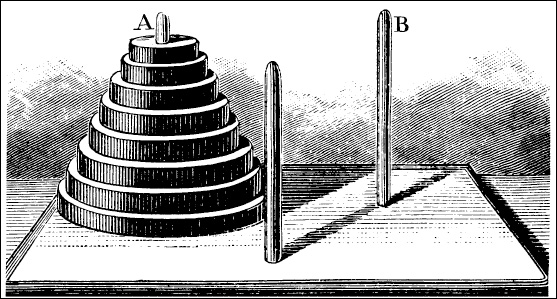
\includegraphics[width=.5\textwidth]{assets/chapter1/Tower of Hanoi}
\end{center}

Mục tiêu của chúng ta, là di chuyển hết tòa tháp sang một trong các cột còn lại, trong đó mỗi lượt chỉ được di chuyển một đĩa từ cột này sang cột khác, và đĩa lớn không bao giờ được đặt trên đĩa nhỏ hơn.

Lucas còn viết một huyền thoại về tòa tháp Brahma khổng lồ, với 64 đĩa làm bằng vàng nguyên chất và ba cột làm từ kim cương.
\marginpar[Làm bằng vàng cơ à. Sao không phải bê tông?]{Làm bằng vàng cơ à. Sao không phải bê tông?}
Ông kể rằng, ngày mà thời gian bắt đầu trôi, Đấng Sáng Thế đã đặt những chiếc đĩa vàng này trên cột thứ nhất, rồi lệnh cho những nhà sư phải chuyển hết số đĩa sang cột thứ ba, theo quy tắc như trên.
Họ làm việc vất vả xuyên cả ngày đêm.
Khoảnh khắc họ đặt chiếc đĩa cuối cùng xuống, tòa Tháp sẽ sụp đổ, và thế giới sẽ đi đến hồi kết.

Không rõ ràng ngay lập tức rằng bài toán này có lời giải, nhưng khi quan sát kỹ hơn (hoặc biết trước bài toán này) sẽ thuyết phục chúng ta rằng nó có. Giờ câu hỏi chính được đưa ra: Chúng ta có thể làm tốt đến đâu? Ta cần ít nhất bao nhiêu lần di chuyển để hoàn thành được bài toán?

Một trong những hướng giải quyết tốt nhất cho những bài toán dạng trên: phương pháp tổng quát hóa. Tòa tháp Brahma có $64$ đĩa còn tòa tháp Hà Tây có $8$ đĩa; vậy ta sẽ tìm hiểu xem chuyện gì sẽ xảy ra nếu ta có $n$ chiếc đĩa.

Một lợi thế của phương pháp này là ta có thể thu nhỏ bài toán hơn nữa. Thực ra, qua cả cuốn sách, ta sẽ thấy sự hiệu quả của việc XÉT NHỮNG TRƯỜNG HỢP NHỎ HƠN trước. Khá dễ dàng để nhận ra cách để di chuyển tòa tháp với 1 hoặc 2 đĩa. Và chỉ cần thử nghiệm nho nhỏ sẽ cho ta thấy được cách tối ưu để giải bài toán với 3 đĩa.

Bước tiếp theo trong việc giải quyết vấn đề: đưa ra các ký hiệu phù hợp: ĐẶT TÊN VÀ CHINH PHỤC. Giả sử $\mathrm{T}_n$ là số lần di chuyển ít nhất để dịch chuyển $n$ cái đĩa từ cột này sang cột khác mà tuân theo luật của Lucas. Vậy hiển nhiên $\mathrm{T}_1 = 1$ và $\mathrm{T}_2 = 3$.

Ta cũng có thể moi được thêm một số thông tin bằng cách xét đến trường hợp nhỏ nhất: Đương nhiên $\mathrm{T}_0 = 0$ vì không bước di chuyển nào cần để chuyển tháp có $0$ đĩa! Những nhà toán học thông thái không bao giờ sợ phải nghĩ quá nhỏ, bởi vì những quy luật tổng quát sẽ dễ nhận thấy hơn khi các trường hợp đặc biệt đã được phân tích kỹ (kể cả khi những trường hợp đấy hiển nhiên).

Nhưng giờ hãy thay đổi cách nhìn của chúng ta và nhìn xa rộng hơn; làm thế nào để di chuyển tòa tháp với nhiều đĩa? Những thử nghiệm với $3$ đĩa chứng tỏ rằng để tối ưu số cách di chuyển, ta sẽ dịch chuyển $2$ đĩa đầu sang cột ở giữa, rồi di chuyển đĩa thứ ba và dịch chuyển $2$ đĩa còn lại. Những nhận xét này gợi ý cho chúng ta cách để dịch chuyển $n$ đĩa một cách tối ưu nhất: Đầu tiên, ta sẽ dịch chuyển $n - 1$ đĩa nhỏ nhất sang cột ở giữa (cần $\mathrm{T}_{n - 1}$ bước), rồi di chuyển đĩa lớn nhất (cần $1$ bước) sang cột thứ ba, và cuối cùng dịch chuyển $n - 1$ đĩa còn lại (cần thêm $\mathrm{T}_{n - 1}$ bước). Như vậy, ta sẽ chuyển được $n$ đĩa (với $n > 0$) qua nhiều nhất $2 \times \mathrm{T}_{n - 1} + 1$ bước:
$$\mathrm{T}_n \le 2 \times \mathrm{T}_{n - 1} + 1, \text{ \ \ \ \ với } n > 0.$$
Công thức trên sử dụng dấu '$\le$' thay vì dấu '$=$' bởi vì cách xử lý của chúng ta chỉ chứng minh $2 \times \mathrm{T}_{n - 1} + 1$ bước là đủ, nhưng ta vẫn chưa chứng minh tại sao $2 \times \mathrm{T}_{n - 1} + 1$ bước là cần để giải quyết bài toán. (Độc giả nào thông minh có thể nghĩ ra cách chứng minh trực tiếp công thức).

\marginpar[Phần lớn các "lời giải" được xuất bản để giải bài toán của Lucas, như lời giải của Allardice và Fraser\href{R. E. Allardice and A. Y. Fraser, La Tour d'Hanoi," Proceedings of the 2. Edinburgh Mathematical Society 2 (1884), 50 - 53}{$^{[7]}$}, đều không chứng minh vì sao $\mathrm{T}_{n} \ge 2 \times \mathrm{T}_{n - 1} + 1$]{Phần lớn các "lời giải" được xuất bản để giải bài toán của Lucas, như lời giải của Allardice và Fraser \href{R. E. Allardice and A. Y. Fraser, La Tour d'Hanoi," Proceedings of the 2. Edinburgh Mathematical Society 2 (1884), 50 - 53}{$^{[7]}$}, đều không chứng minh vì sao $\mathrm{T}_{n} \ge 2 \times \mathrm{T}_{n - 1} + 1$}

Nhưng ta có thể tìm cách nào tốt hơn không? Thực ra là không. Đến một lúc nào đó ta sẽ phải di chuyển cái đĩa ở đáy. Khi ta làm thế, $n - 1$ đĩa đầu phải ở trên phải ở cùng một cột nào đó, và nó sẽ mất ít nhất $\mathrm{T}_{n - 1}$. Nếu không cảnh giác, ta có thể di chuyển đĩa lớn nhất nhiều hơn 1 lần. Nhưng sau khi di chuyển đĩa lớn nhất lần cuối cùng, ta cần dịch chuyển lại tất cả $n - 1$ đĩa còn lại (nhớ là tất cả đĩa này phải trên cùng 1 cột) lên trên thằng lớn nhất; bước này cũng cần ít nhất $\mathrm{T}_{n - 1}$ bước. Vì thế, nên:
$$\mathrm{T}_n \ge 2 \times \mathrm{T}_{n - 1} + 1, \text{ \ \ \ \ với } n > 0.$$
Hai bất đẳng thức này, cùng với đáp án hiển nhiên với $n = 0$, cho ta:
\begin{equation}\label{eq:1.1}
    \begin{aligned}
        & \mathrm{T}_0 = 0; \\
        & \mathrm{T}_n = 2 \times \mathrm{T}_{n - 1} + 1, \text{ \ \ \ \ với } n > 0.
    \end{aligned}
\end{equation}
(Để ý rằng công thức trên đúng với những giá trị ta đã biết như $\mathrm{T}_1 = 1$ hay $\mathrm{T}_2 = 3$. Kinh nghiệm của chúng ta với những trường hợp nhỏ lẻ không những giúp chúng ta trong việc tìm ra công thức tổng quát, mà nó còn là công cụ tiện lợi để kiểm tra xem ta có mắc phải sai lầm chết người nào không. Những công cụ kiểm tra như thế này rất đáng giá khi ta đi sâu vào những kỹ thuật phức tạp hơn ở chương sau.)

Những tập hợp các biểu thức như \eqref{eq:1.1} được gọi là
\marginpar[Ừ, hình như mình nhìn thấy từ này rồi]{Ừ, hình như mình nhìn thấy từ này rồi}
công thức truy hồi. Chúng cho ta các giá trị tại biên và những biểu thức để tính giá trị tổng quát thông qua các giá trị trước. Đôi khi ta chỉ gọi một mình biểu thức là công thức truy hồi, dù cho thực tế nó cần giá trị biên để trở thành một công thức truy hồi. 

Công thức truy hồi có thể giúp chúng ta tính được $\mathrm{T}_n$ với mọi $n$ ta muốn. Nhưng không ai thich tính toán bằng công thức truy hồi cả;  đặc biệt khi $n$ khá lớn, nó sẽ tốn rất nhiều thời gian. Công thức truy hồi cũng chỉ thể hiện những thông tin gián tiếp và địa phương, không có tính tổng quát. Một thứ có thể giúp ta tránh khỏi những vấn đề này chính là \textit{giải pháp cho công thức truy hồi}. Đó chính là một công thức đẹp, gọn, còn gọi là "dạng đóng" của $\mathrm{T}_n$ để chúng ta có thể tính toán nhanh, ngay cả cho giá trị lớn của $n$. Với "dạng đóng" của $\mathrm{T}_n$, ta sẽ hiểu được bản chất của $\mathrm{T}_n$ là gì.

Vậy làm thế nào để chúng ta giải được công thức truy hồi này? Một cách ta có thể dùng là đoán đáp án, sau đó chứng minh rằng đáp án của chúng ta đúng. Và hy vọng lớn nhất của ta trong việc đoán đáp án chính là xét các trường hợp nhỏ của công thức truy hồi. Vậy ta tính toán được lần lượt, $\mathrm{T}_3 = 2 \times 3 + 1 = 7$, $\mathrm{T}_4 = 2 \times 7 + 1 = 15$, $\mathrm{T}_5 = 2 \times 15 + 1 = 31$, $\mathrm{T}_6 = 2 \times 31 + 1 = 63$. Ô! Nhìn như nó theo công thức:
\begin{equation}\label{eq:1.2}
    \begin{aligned}
        & \mathrm{T}_n = 2^n - 1, \text{ \ \ \ \ với } n > 0.
    \end{aligned}
\end{equation}
Ít nhất nó đúng với $n \le 6$.


\textit{Quy nạp} 
\marginpar[Quy nạp chứng minh rằng ta có thể trèo lên cao đến tùy thích cứ như chúng ta đang trên một chiếc thang, bằng cách chứng minh rằng ta có thể trèo lên bậc thấp nhất (cơ sở) và từ đó chứng minh với mỗi bậc tiếp theo ta có thể leo đến bặc tiếp theo nữa (quy nạp)]{Quy nạp chứng minh rằng ta có thể trèo lên cao đến tùy thích cứ như chúng ta đang trên một chiếc thang, bằng cách chứng minh rằng ta có thể trèo lên bậc thấp nhất (cơ sở) và từ đó chứng minh với mỗi bậc tiếp theo ta có thể leo đến bặc tiếp theo nữa (quy nạp)} 
là một trong những cách tổng quát để chứng minh rằng một nhận định nào đó về số nguyên $n$ đúng với mọi $n \ge n_0$. Đầu tiên ta chứng minh nhận định đúng khi n đặt giá trị nhỏ nhất, $n_0$, đây được gọi là bước cơ sở. Tiếp theo, ta chứng minh nhận định đúng với $n > n_0$, giả sử nhận định đã được chứng minh đúng với mọi giá trị từ $n_0$ đến $n - 1$; đây được gọi là bước quy nạp. Dạng chứng minh như thế này cho ta vô tận kết quả chỉ trong hữu hạn bước làm.



Các dạng bài giải công thức truy hồi rất lý tưởng cho cách chứng minh bằng quy nạp. Ở ví dụ của ta, ta có thể suy luận ra \eqref{eq:1.2} khá dễ dàng từ \eqref{eq:1.1}: Bước cơ sở hiển nhiên đúng, do $\mathrm{T}_0 = 2^0 - 1 = 0$. Và qua bước quy nạp, ta tiếp tục chứng minh khẳng định đúng với $n > 0$ nếu ta giả sử \eqref{eq:1.2} đúng khi n được thay thế bởi $n - 1$:
$$\mathrm{T}_n = 2 \times \mathrm{T}_{n - 1}  + 1 = 2 \times (2^{n - 1} - 1) + 1 = 2^n - 1.$$
Vậy \eqref{eq:1.2} đúng với $n$. Tuyệt! Hành trình đi tìm $\mathrm{T}_n$ của chúng ta đã thành công mỹ mãn.

Tất nhiên công việc của các nhà sư vẫn chưa kết thúc; họ vẫn đang phải miệt mài di chuyển những cái đĩa, và sẽ di chuyển những cái đĩa này khá lâu, do với $n = 64$ thì ta sẽ có $2^64 - 1$ bước (tầm khoảng 18 tỷ tỷ bước). Kể cả với tốc độ thần kỳ $1$ bước mỗi nano giây, họ sẽ phải tốn hơn 5 thiên niên kỷ chỉ để dịch chuyển tòa tháp Brahma. Bài toán gốc của Lucas dễ thở hơn một chút. Nó chỉ cần $2 ^ 8 - 1 = 255$ bước, sẽ mất khoảng 4 phút nếu nhanh tay.

Công thức truy hồi trong bài toán tháp Hà Tây khá điển hình trong những dạng có nhiều ứng dụng trong toán học. Khi đi tìm "dạng đóng" của một đại lượng nào đó ta quan tâm như $\mathrm{T}_n$, ta cần đi qua 3 bước:
\begin{enumerate}
    \item Xét các trường hợp bé trước. Làm thế giúp chúng ta có cái nhìn sâu sắc hơn về vấn đề và giúp ta ở bước 2 và 3.
    \item Tìm và chứng minh 
    \marginpar[Chứng minh là gì? "Một nửa của một phần trăm rượu nguyên chất"]{Chứng minh là gì? "Một nửa của một phần trăm rượu nguyên chất"}
    một biểu thức toán học cho đại lượng ta quan tâm. Với bài toán tháp Hà Tây, đó là công thức truy hồi \eqref{eq:1.1} giúp ta có thể tính được $\mathrm{T}_n$ với mọi $n$.
    \item Tìm và chứng minh "dạng đóng" của biểu thức của chúng ta. Với bài toán tháp Hà Tây, đó chính là \eqref{eq:1.2}
\end{enumerate}
Bước thứ ba sẽ là bước ta sẽ tập trung nhiều qua cả quyển sách. Thực ra, ta sẽ thường xuyên bỏ qua bước 1 và 2, vì ta sẽ có công thức truy hồi qua các biểu thức toán học ngay từ đầu. Nhưng ngay cả thế, ta sẽ làm rất nhiều các bài toán con mà sẽ đưa ta qua cả 3 bước.

Nghiên cứu của ta về tháp Hà Tây đã dẫn chúng ta đến với kết quả đúng, nhưng ta vẫn cần một "phép màu quy nạp"; ta vẫn phải dựa vào những dự đoán đầy may rủi của mình. Một trong những mục tiêu hàng đầu của quyển sách này chính là giải thích vì sao một người có thể giải quyết những công thức truy hồi mà không cần đến tâm linh. Ví dụ, ta có thể đơn giản hóa công thức truy hồi \eqref{eq:1.1} bằng cách cộng thêm $1$ vào cả hai vế của biểu thức:

\begin{equation*}
    \begin{aligned}
        & \mathrm{T}_0 + 1 = 1 \\
        & \mathrm{T}_n + 1 = 2 \times \mathrm{T}_{n - 1} + 2, \text{ \ \ \ \ với } n > 0. \\ 
    \end{aligned}
\end{equation*}
\marginpar[Thật thú vị! Ta ẩn đi hệ số $\mathbf{+1}$ trong \eqref{eq:1.1} bằng cộng thêm phần tử thay vì trừ nó đi]{Thật thú vị: ta ẩn đi hệ số $\mathbf{+1}$ trong \eqref{eq:1.1} bằng cộng thêm phần tử thay vì trừ nó đi}
Bây giờ nếu ta đặt $\mathrm{U}_n = \mathrm{T}_n + 1$, ta có:
\begin{equation}\label{1.3}
    \begin{aligned}
        & \mathrm{U}_0 = 1 \\
        & \mathrm{U}_n = 2 \times \mathrm{U}_{n - 1}, \text{ \ \ \ \ với } n > 0.
    \end{aligned}
\end{equation}
Thực sự không cần là thiên tài cũng thấy được dạng tổng quát của công thức truy hồi này: $\mathrm{U}_n = 2^n$; do vậy $T_n = 2^n - 1$. Ngay cả máy tính cũng suy luận ra được điều đó.